\section{Introducción}

Comencemos con un problema de cargas. Sean $q_1$ y $q_2$ dos cargas positivas, por ejemplo dos protones que se encuentran en una situación de equilibrio. Y ahora introducimos una carga negativa, por ejemplo un electrón $e$ con una velocidad $V_0$. ¿Qué va a ocurrir en el sistema? ¿Cuál va a ser la trayectoria del electrón? ¿Cómo modelizamos matemáticamente un ejemplo tan sencillo? ¿Cómo solucionamos esa modelización? ¿Ocurrre algo similar dentro de los cables eléctricos?

\begin{wrapfigure}{l}{0.4\textwidth}\vspace{-0.9cm}\begin{center}
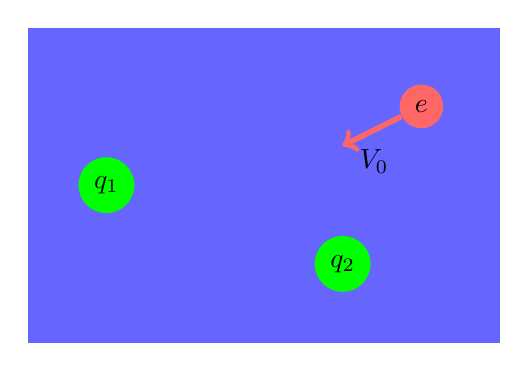
\begin{tikzpicture}
\fill[blue!60]
(0,0) rectangle (6,4);
\path[draw]  (1,2)node[circle,fill=green] (nodeA) {$q_1$};
\path[draw]  (4,1)node[circle,fill=green] (nodeB) {$q_2$};
\path[draw]  (5,3)node[circle,fill=red!60] (nodeC) {$e$};
%\draw[->] (-2,3)--(-1,3);
\draw[->,line width=2pt,red!60] (nodeC) -- (4,2.5);
\path[draw]  (4.4,2.3)node {$V_0$};
\end{tikzpicture}

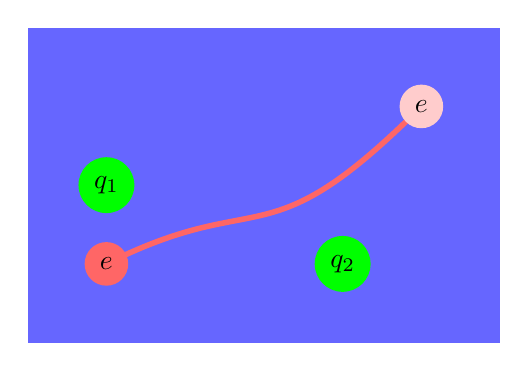
\begin{tikzpicture}
\fill[blue!60]
(0,0) rectangle (6,4);
\path[draw]  (1,2)node[circle,fill=green] (nodeA) {$q_1$};
\path[draw]  (4,1)node[circle,fill=green] (nodeB) {$q_2$};
%\path[draw]  (5,3)node[circle,fill=red!60] (nodeC) {$e$};
\draw[line width=2pt,red!60] (5,3).. controls (3,1) and (3,2) ..(1,1);
\path[draw]  (5,3)node[circle,fill=red!20] (nodeC) {$e$};
\path[draw]  (1,1)node[circle,fill=red!60] (nodeC) {$e$};
%\draw[->,line width=2pt,red!60] (nodeC) -- (4,2.5);
\end{tikzpicture}
\end{center}
\end{wrapfigure}

Todas estas preguntas son las que vamos a dar respuesta en este artículo. nos enfrentaremos a una ecuación diferencial cuya solución definirá la trayectoria del electrón que introducimos en el sistema de equilibrio. Veremos que llegar a una solución exacta es algo que en la mayoría de los casos no se podrá dar. Veremos que otras herramientas tendremos para poder conseguir al menos una solución apróximada y analizaremos con detalle estas soluciones. Esperemos se diviertan y aprendan mucho con este artículo.


%\begin{figure}
%\begin{figurebox}\centering
%\includegraphics[scale=0.35]{Bernoulli.jpg}
%\includegraphics[scale=0.4]{hamer .jpg}  encontrar a este hombre a la web
% \includegraphics[scale=0.1]{william.jpg}

% \includegraphics[scale=1.18]{Anderson.jpg} 
%\includegraphics[scale=0.49]{Ronald_Ross.jpg} \caption{De izquierda a derecha: Bernoulli, A.G. McKendrick, W.O. kermack y R. Ross}
%\end{figurebox}
%\caption{De izquierda a derecha: Bernoulli, A.G. McKendrick, W.O. kermack y R. Ross}
%\end{figure}
\section{Modelo matemático de de la trayectoria del electrón}
Para modelizar la trayectoria del electrón, o en general una partícula,  introducido en un sistemas de partículas (que pueden ser electrones o protones) necesitamos determinar:
\begin{itemize}
\item Su posición $x(t)=(x_1(t),x_2(t))$ en el instante $t$ sabiendo que su posición inicial es  $x(0)=x_0=(x_{10},x_{20})$ .
\item Su velocidad $V(t)=(V_1(t),V_2(t))$ en el instante $t$ sabiendo que su velocidad inicial es $V(0)=V_0$.
\item Su aceleración $a(t)$ en el instante $t$.
\end{itemize}
Es bien conocido que la derivada del espacio es la velocidad y que la derivada de la velocidad es la aceleración. De este modo podemos plantear el siguiente sistema diferencial:
\begin{equation}\label{eq:mov}
\left.\begin{array}{r}
x'(t)=V(t)\\
V'(t)=a(t)\\
\end{array}\right\}
\end{equation}
La pregunta clave ahora para poder formular completamente nuestro sistema de ecuaciones diferenciales es, ¿cuánto vale la aceleración $a(t)$ en cada instante? Y la respuesta la tenemos por la ecuación fundamental de la dinámica que nos dice que la fuerza es el producto de la masa por la aceleración, esto es $F=m\cdot a$. Esta ecuación proviene de la segunda ley de Newton\footnote{Mutationem motus proportionalem esse vi motrici impressæ, \& fieri secundum lineam rectam qua vis illa imprimitur.}.

Usando lo anterior la función $a(t)$ puede ser calculada conociendo la fuerza $F$ que será la suma de las fuerzas ejecutada entre el electrón y los dos protones en equilibrio y la masa $m_e$ del electrón. Este razonamiento se puede realizar en genérico introduciendo una partícula en un sistema en equilibrio que contiene $n$ partículas pero vamos a realizar el estudio con un electrón que se introduce en un sistema equilibrado donde hay dos protones. Generalizarlo es bastante sencillo y lo dejamos como ejercicio para el lector. 

Sabemos que la fuerza entre dos cargas...
  
\section{Resolución numérica: Método de Euler}
Como hemos mencionado antes, llegar a una solución analítica de un sistema de ecuaciones diferenciales es complicado. Existen casos donde esto si ocurre, por ejemplo la caida libre. Supongamos un objeto de masa $m$ a una altura $h$, las ecuaciones de movimiento de caída libre vendrían modelizadas con el sistema de ecuaciones (\ref{eq:mov}). La aceleración en este caso se corresponde con la aceleración de la gravedad, esto es $g=9.81$  
\begin{wrapfigure}{l}{0.15\textwidth}\vspace{-0.9cm}
\begin{center}
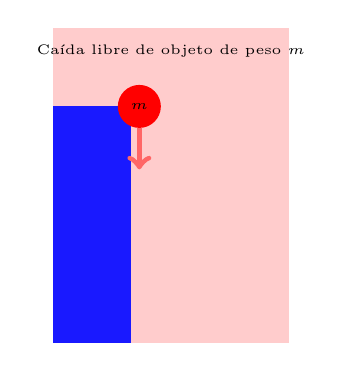
\begin{tikzpicture}
%\path[draw]  (1,2.4)node (nodeA) {\tiny Caída libre de objeto de peso $m$};
\fill[red!20] (0,0) rectangle (3,4);
\fill[blue!90](0,0) rectangle (1,3);
\path[draw]  (1.1,3)node[circle,fill=red] (nodeA) {\tiny $m$};
\draw[->,line width=2pt,red!60] (nodeA) -- (1.1,2.2);
\path[draw]  (1.5,3.7)node (nodeA) {\tiny Caída libre de objeto de peso $m$};
\end{tikzpicture}

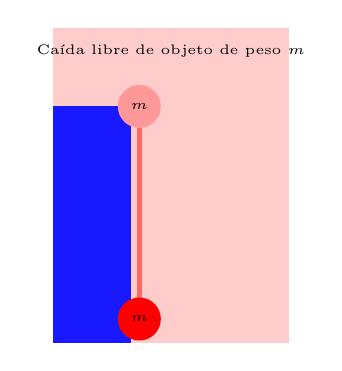
\begin{tikzpicture}
%\path[draw]  (1,2.4)node (nodeA) {\tiny Caída libre de objeto de peso $m$};
\fill[red!20] (0,0) rectangle (3,4);
\fill[blue!90](0,0) rectangle (1,3);
\path[draw]  (1.1,3)node[circle,fill=red!40] (nodeA) {\tiny $m$};
\draw[-,line width=2pt,red!60] (nodeA) -- (1.1,0.1);
\path[draw]  (1.1,0.3)node[circle,fill=red] (nodeA) {\tiny $m$};
\path[draw]  (1.5,3.7)node (nodeA) {\tiny Caída libre de objeto de peso $m$};
\end{tikzpicture}
\end{center}
\end{wrapfigure}



\section{Resolución numérica de nuestra ecuación}

\section{Fallos cualitativos de Euler. Mejoras.}

%\bibliographystyle{plain}
%\bibliography{catenaria}



\newpage
%%% Local Variables: 
%%% mode: latex
%%% TeX-master: "matematicaseningenieria"
%%% End: 
